\chapter{Sequenz Diagramm}
\section{Erstellen einer neuen Challenge}
In diesem Diagramm sehen wir das detaillierte Klassen Diagramm für die User unseres Tools:
\begin{figure}[H]
\centering

\includegraphics[width=1\textwidth]{../SequenzDiagramm/CreateChallangeCorrected.png}
\caption{Sequenz Diagramm Challenge}
\end{figure}
Dieses Sequenz Diagramm beschreibt den Ablauf und die genutzten Klassen wenn der User eine neue Challenge erstellt.

\section{Noch kein Journal Eintrag für den heutigen Tag}
\begin{figure}[H]
\centering
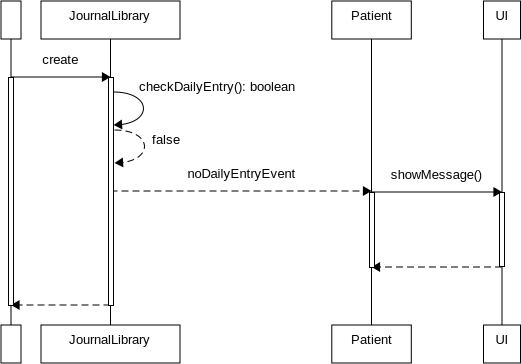
\includegraphics[width=1\textwidth]{../SequenzDiagramm/NoEntryCorrected.png}
\caption{Sequenz Diagramm Journaleintrag}
\end{figure}
Dieses Sequenz Diagramm zeigt wie nach dem Login, beim erstellen der Journal Library, überprüft wird ob der User für den heutigen Tag bereits einen Journal Eintrag erstellt hat. Falls nicht wird auf dem UI eine Meldung angezeigt.
